\documentclass[11pt]{article}


\usepackage{graphicx}
\usepackage{epsfig} % for postscript graphics
\usepackage[usenames]{color}
\usepackage{amssymb}
\usepackage{epstopdf}
\usepackage{amsfonts}
\usepackage{amsmath}
\usepackage{natbib}
\usepackage{eca_molecolres}
\usepackage{xspace}
\usepackage{mathrsfs}
\usepackage{array}
\usepackage{multirow}
\usepackage{rotating}
\usepackage{enumerate}
\usepackage[draft]{hyperref}
\usepackage[nolists,tablesfirst]{endfloat}
\usepackage{url}
\usepackage{scalerel}




\newcommand{\relat}{R}
\newcommand{\relatset}{\mathscr{R}}
\newcommand{\nA}{\mathcal{A}}
\newcommand{\nL}{\mathcal{L}}
\newcommand{\nG}{\mathcal{G}}

\newcommand{\Pe}{\mathrm{P}_\epsilon}
\newcommand{\PR}{\mathrm{P}_\relat}

\newcommand{\bkappa}{\bm{\kappa}}

\newcommand{\comment}[1]{\textcolor{red}{#1}}

\newcommand{\BY}{\mathbf{Y}}
\newcommand{\BX}{\mathbf{X}}
\newcommand{\I}{\mathbb{1}}
\newcommand{\bomega}{\bm{\omega}}

\newcommand{\Exp}{\mathbb{E}}

\newcommand{\founders}{\mathscr{F}}
\newcommand{\nonfound}{\mathscr{N}}
\newcommand{\nonfounds}{\mathscr{N}_s}
\newcommand{\nonfounde}{\mathscr{N}_e}
\newcommand{\nonfoundse}{\mathscr{N}_{s,e}}

\newcommand{\gscramble}{{\sc gscramble}}
\newcommand{\BC}{BC}


\usepackage{subcaption}
\captionsetup[subfigure]{position=top, singlelinecheck=off, labelfont=bf, justification=raggedright, font=singlespacing} 




%%%%%%%%%%%%%%%%%%%%%%%%%%%%%%%%%%%
%% A bunch of Mol Ecol Res Formatting
% change the way captions are displayed beneath figures (Only display figure number)
\makeatletter
\renewcommand{\@makecaption}[2]{{\centering   \vskip\abovecaptionskip \bfseries #1} #2}
\newcommand{\@makecaptionZ}[2]{%
  \vskip\abovecaptionskip
  \sbox\@tempboxa{#1}%
  \ifdim \wd\@tempboxa >\hsize
    #1\par
\else
\global \@minipagefalse
\hb@xt@\hsize{\hfil\box\@tempboxa\hfil}%
\fi
\vskip\belowcaptionskip}
\makeatother

%% change section heading styles
\makeatletter
\renewcommand\section{\@startsection {section}{1}{\z@}%
                                   {-3.5ex \@plus -1ex \@minus -.2ex}%
                                   {1.5ex \@plus 0ex}%
                                   {\normalfont\normalsize\bfseries}}
\renewcommand\subsection{\@startsection{subsection}{2}{\z@}%
                                     {-3.25ex\@plus -1ex \@minus -.2ex}%
                                     {1.5ex \@plus .2ex}%
                                     {\normalfont\normalsize\itshape}}
\renewcommand\subsubsection{\@startsection{subsection}{2}{\z@}%
                                     {-3.25ex\@plus -1ex \@minus -.2ex}%
                                     {1.5ex \@plus .2ex}%
                                     {\normalfont\footnotesize\bfseries}}
\makeatother



\setcitestyle{aysep={}}
\AtBeginDelayedFloats{\renewcommand{\baselinestretch}{1.6}}


\textwidth = 6.5 in
\textheight = 8.622 in
\oddsidemargin = 0.0 in
\evensidemargin = 0.0 in
\topmargin = 0.378 in
\headheight = 0.0 in
\headsep = 0.0 in
\parskip = 0.2in
\parindent = 0.0in


%!TEX root = main.tex


%%%%% THIS IS THE SECTION WHERE THE AUTHOR PUTS IN ALL OF THEIR TITLE AND AFFILIATION
%%%%% INFORMATION AND  A FEW OTHER THINGS
\newcommand{\myTitle}{{\sc gscramble:} Simulation of admixed individuals without reuse of genetic material}
\title{\myTitle}

% redefine this to make author list. Note affiliation symbols are done manually.
% All caps tends to look better
\newcommand{\myAuthors}{Eric C. Anderson$^{*,\dagger,\ddag,\S}$, Rachael M. Giglio$^{\#}$, Matthew G. DeSaix$^{\ddag,\#}$ Timothy J. Smyser$^{\#}$}
\author{Eric C. Anderson$^{*,\dagger,\ddag,\S}$, Rachael M. Giglio$^{\#}$, Matthew G. DeSaix$^{\ddag,\#}$ Timothy J. Smyser$^{\#}$}


% redefine to make the affiliation list.  Note symbols are done manually
\newcommand{\myAffiliations}{$^*$Fisheries Ecology Division,
    Southwest Fisheries Science Center, National Marine Fisheries Service, NOAA,
    110 McAllister Road,
    Santa Cruz, CA 95060, USA.,
    $^\dagger$Dept. of Fish, Wildlife, and Conservation Biology, Colorado State University, Fort Collins, CO, USA,
    $^\ddag$Dept. of Biology, Colorado State University, Fort Collins, CO, USA,
    $^\#$National Wildlife Research Center, United States Department of Agriculture, Wildlife Services,
    Fort Collins, CO, USA
}
\renewcommand{\AuthorAddresses}{\myAffiliations}

\renewcommand{\KeyWords}{genetic stock identification, mixture deconvolution, permutation testing, power analysis, R package}

\renewcommand{\CorrespondingAuthor}{Eric C. Anderson, eric.anderson@noaa.gov}


% the email address for the corresponding author
\newcommand{\myEmailAddress}{eric.anderson@noaa.gov}
\newcommand{\myEmailFootnote}{$^\S$}

% here you can put your very own copyright notice
\newcommand{\myCopyright}{}

% here you can put a running title (a short title that goes on the left of the
% even pages)
\newcommand{\myRunningTitle}{Linkage-aware power assessment for admixture proportions}
\renewcommand{\RunningTitle}{\myRunningTitle}

% and here you put the running author (short listing of authors for the
% upper right header on the odd pages)
\newcommand{\myRunningAuthor}{Anderson {\em et al.}}

%%%% DONE WITH AUTHOR/TITLE/ETC INFORMATION DEFINITION


% let \cite be the same as \citep
\renewcommand{\cite}{\citep}

\setlength{\parindent}{2em}

%%%%%%%%%%%%%%%%%%%%%%%%%%%%%%%%%%%%%%%%%%%%%%%%%%%%%%

\textwidth=6.5in \textheight= 8.0in \evensidemargin=0in
\oddsidemargin=0in
\parskip=.2ex


%% some handy things for making bold math
\def\bm#1{\mathpalette\bmstyle{#1}}
\def\bmstyle#1#2{\mbox{\boldmath$#1#2$}}
\newcommand{\thh}{^\mathrm{th}}


%% Some pretty etc.'s, etc...
\newcommand{\cf}{{\em cf.}\xspace }
\newcommand{\eg}{{\em e.g.},\xspace }
\newcommand{\ie}{{\em i.e.},\xspace }
\newcommand{\etal}{{\em et al.}\ }
\newcommand{\etc}{{\em etc.}\@\xspace}




% in this document if you say \sometimes{\acaption} then 
% it returns nothing.
\newcommand{\sometimes}[1]{}




\begin{document}



\renewcommand{\baselinestretch}{1.66}
\normalsize

\maketitle

\begin{abstract}
%!TEX root = main.tex


While a best practice for evaluating the behavior of genetic clustering algorithms 
on empirical data is to conduct parallel analyses on simulated data, these types 
of simulation techniques often involve sampling genetic data with replacement. 
In this paper we demonstrate that sampling with replacement, especially with large 
marker sets, inflates the perceived statistical power to correctly assign individuals
(or the alleles that they carry)
back to source populations---a phenomenon we refer to as resampling-induced, 
spurious power inflation (RISPI). To address this issue, we present \gscramble{}, a 
simulation approach in R for creating biologically informed individual genotypes from 
empirical data that: 1) samples alleles from populations \textit{without} replacement and 
2) segregates alleles based on species-specific recombination rates. This framework
makes it possible to simulate admixed individuals in a way that respects the physical
linkage between markers on the same chromosome and which does not suffer
from RISPI.  This is achieved in \gscramble{} by allowing 
users to specify pedigrees of varying complexity 
in order to simulate admixed genotypes, segregating and tracking haplotype blocks 
from different source populations through those pedigrees, and then sampling---using
a variety of permutation schemes---alleles from empirical data into those haplotype blocks.
We demonstrate the functionality of 
\gscramble{} with both simulated and empirical data sets and highlight additional uses of 
the package that users may find valuable.
\end{abstract}

%!TEX root = main.tex

\section*{Introduction}

Genetic clustering algorithms are commonly used to describe genetic structure among populations, reflecting the cumulative 
effects of isolation, connectivity (i.e., genetic migration), selection, and genetic drift.  The ability of such algorithms to differentiate populations 
is limited by the extent of genetic differentiation among populations and the capacity to resolve those differences given the available marker 
set and sample sizes from the respective populations.  Based on an initial description of genetic structure, ecologists are frequently 
interested in describing patterns of genetic movement among populations, often inferred from the mismatch between the sampling location 
and genetic origins of a given individual \citep{paetkau1995microsatellite,wilson2003bayesian}.  Genetic movement has many implications, 
such as influencing evolutionary processes, maintaining genetic variation through gene flow, and driving disease dynamics 
\citep{huestis2019windborne} and affecting patterns of invasive species expansion CITE.

In using clustering algorithms to describe genetic structure among natural populations, researchers frequently identify individuals of 
mixed ancestry---
characterized as individuals with proportions of their genome attributed to multiple subpopulations, sensu \citet{pritchard2000inference}.
a trait often summarized as the proportion of an individual’s genome originating from each of $K$ subpopulations, sensu 
\citet{pritchard2000inference}.  Various processes could contribute to such mixed associations.  Most directly, individuals may represent the 
influences of gene flow among populations, occurring in recent or prior generations, with the observed complex ancestry patterns accurately 
representing contributions from multiple sampled populations.  However, similar patterns may result from functionally different patterns of 
population structuring.  For example, such patterns might be expected when clinal systems governed by isolation by distance are described 
as discrete genetic clusters.
NOTE I think a line here about exogenous immigrants might be worthwhile to set up 2 biological processes paired with a statistical process, 
something like END NOTE
Alternatively, individuals of mixed ancestry could reflect immigration from outlying populations (e.g., exogenous immigration), with true source 
populations not sufficiently
represented in the sample to be among the characterized $K$ subpopulations.
Furthermore, the characterization of admixed individuals may reflect a limitation of the statistical power of the genetic data,
as a function of both the marker set and sample size, to resolve the true underlying patterns of genetic structure.
 The challenge for researchers then becomes correctly identifying the ecological and/or statistical processes by which observed complex 
 ancestry patterns were created.

A best practice for evaluating the behavior of genetic clustering algorithms on an empirical dataset is to conduct
parallel analyses on simulated data where the truth is known, structured to mirror the empirical data set
as closely as possible \citep{vaha2006efficiency,anderson2008improved,latch2011fine}.
Techniques to simulate individual genotypes in this context frequently use sampling with replacement from the
observed allele frequencies (see CITE, CITE, CITE).
However, sampling with replacement implicitly increases the pairwise genetic distance among simulated samples, relative to the observed 
samples, and
inflates the perceived ability to correctly assign individuals back to source populations. \citet{anderson2008improved}
documented this type of artifact in the context of simulations to assess the power for
genetic stock identification (GSI), a type of clustering application in which individuals are constrained to have
all their ancestry from a single subpopulation.
We demonstrate, below, that similar artifacts occur when simulating data to
assess how accurately admixture fractions can be estimated.  We refer to this phenomenon as resampling-induced
power inflation, or RIPI for short.
NOTE I would proposed holding on to the next sentence as we build the idea of mixed ancestry in the next paragraph END NOTE
In this study, we additionally develop and illustrate an approach by which RIPI can be eliminated
from simulations by constraining the genetic differences among simulated populations to match
those of populations from which the samples were obtained.

Beyond simply evaluating the resolution of discrete populations in a simulated framework, researchers may also be
interested in how individuals of admixed ancestry are genetically characterized given the statistical power of the available dataset and the 
analysis methods used.
Recognizing that connectivity among genetically distinct populations may be relatively rare, additional insight into the
frequency of immigration can be gained by integrating across generations to identify both direct migrants and descendants of migrants
 (i.e., F1 hybrids or advanced hybrids reflecting the effect of backcrossing across multiple generations [BC1, \ldots,
BCX]).
However, the process of recombination during meiosis creates a distribution of expected associations to parental populations among
advanced hybrid classes.
Treating linked loci as independent can lead to the false interpretation that the association of advanced hybrid classes to parental population 
occur strictly as discrete distributions.
Therefore, in evaluating descendants of migrants within a simulated framework, it is imperative to take into consideration the pattern of
linkage among loci available for analysis.

In response to these needs, we developed \gscramble{} – a simulation approach that samples alleles from respective populations without 
replacement, thus maintaining the genetic differences in the empirical dataset.
Further, by simulating individual genotypes based on user-defined pedigrees, \gscramble{} allows for the simulation of admixed genotypes of 
varying degrees of complexity while allowing the tracking of haplotype blocks from source populations within the specified pedigree.
By integrating species-specific recombination rates, \gscramble{} simulates biologically informed genotypes that mirror empirical data.
We develop and illustrate \gscramble{} with use of single nucleotide polymorphic (SNP) genotypes.




\section*{Methods}

\subsection*{An introductory motivating example}


Before we proceed to a description of the methodology used by \gscramble{},
we demonstrate a case in which using a standard sampling-with-replacement
approach induces RIPI when estimating admixture fractions.
To construct this simple example, we used the R programming language \citep{Rcoreteam} to
simulate allele frequencies for $L$ biallelic
loci in a single population from a $\mathrm{Beta}(1, 8)$ distribution and then simulated
two samples, $A$ and $B$, each of size $N$ diploid genotypes. The genotypes in $A$ and $B$ were simulated
from the same allele frequencies assuming Hardy-Weinberg equilibrium.

In this case,
each set of $N$ individuals is a sample from exactly the same population, so
there is clearly no basis for performing population assignment between $A$ and $B$;
however, we treated samples $A$ and $B$ as if they were sampled from two potentially different
populations, and simulated $9n$ new individuals: $n$ new individuals at each of the 9 values of
$q_A$, the admixture fraction for population $A$, in  $\{0, \frac{1}{8}, \frac{1}{4}, \frac{3}{8}, \frac{1}{2}, \frac{5}{8}, \frac{3}{4}, \frac{7}{8}, 1\}$. 
We simulated these genotypes according to the "admixture model" used in {\em structure} \citep{pritchard2000inference}.  Briefly, at each 
locus, independently, the origin
of each gene copy was simulated to be from
population $A$ with probability $q_A$ and from population $B$ with probability $1-q_A$.  Subsequently,
the allelic types of gene copies from $A$ ($B$), at a locus, were simulated by sampling with replacement
from the alleles at that locus in sample $A$ ($B$).
We then added these $9n$ simulated individuals to the $N$ original individuals  from $A$ and $N$ from $B$
and analyzed all the genotypes using ADMIXTURE with $K=2$. On each data set we performed a supervised analysis in which the original 
$N$ samples from each
population were provided as learning samples, and also an
unsupervised analysis when the origin of the samples from $A$ and $B$ were regarded as unknown.

For each combination of $L \in \{10^2, 10^3, 10^4, 10^5\}$,
$N \in \{25, 50, 100, 250\}$ and $n\in\{3,12,24\}$ we conducted multiple replicates
of the entire process of
simulating samples $A$ and $B$, simulating the $9n$ additional individuals, and
then analyzing them with ADMIXTURE.  We conducted $R$ replicates so that,
for each combination of $L$, $N$, and $n$ we had simulated $Rn=480$ new individuals
at each $q_A$ value; thus, $R=160$ replicates when $n = 3$, $R=40$ when $n=12$, and
$R=20$ when $n=24$.


Because the simulations were done in a na\"{i}ve way that effectively assumes that the population
allele frequencies are identical to those observed in the samples themselves, we hypothesized that ADMIXTURE would return estimates of 
$q_A$ that were
centered around the true values, even though samples $A$ and $B$ were drawn from the same
population.
We further expected that ADMIXTURE would return more accurate estimates of
$q_A$ when $N$ was smaller and the number of loci was larger.
We summarized the results by plotting boxplots of the ADMIXTURE-inferred $q_A$ values,
 for the 480 newly simulated individuals (and for the original samples, $A$ and $B$, in the
 case of unsupervised clustering),
for each combination of $L$, $N$, and $n$.




\subsection*{Genomic Simulation Pedigrees}

Our approach for simulating admixed individuals without inflating perceived power for
the estimation of their admixture fractions is motivated by the traditional cross-validation
approach for evaluating the power of mixture proportion
estimation in genetic stock identification (e.g., the cross-validation approach
desribed in \citealt{moran2019bayesian}).
In the cross-validation approach, individuals are removed from the reference
samples and placed in a mixture sample of "unknowns", whose origin
is inferred using the remaining individuals in the reference samples.  A key
feature of this approach is that no new genetic material is being created by
sampling with replacement; however the genetic material of all individuals
in the original samples is being used---either within the remaining individuals in the
reference samples or within the individuals in the mixture.

Our scheme, described here, extends the traditional cross-validation approach
by simulating the descent of chunks of chromosome through a user-specified
pedigree to create admixed individuals.  By imposing certain constraints
on the pedigree, our framework ensures that all the genetic material
within the original individuals is used to either create admixed individuals or to
remain within reference individuals (i.e., those that are purely of one
putative subopulation), and yet no new genetic material is
created by sampling with replacement from the original samples.

We call the structure
we use to do this sort of cross-validation simulation of admixed individuals
a {\em genomic simulation pedigree} or GSP.  Like any pedigree,
a GSP includes a set of founders (individuals that have no parents specified in the
pedigree), and it includes non-founders; however, we introduce an additional node
type in the GSP that represents samples taken from the non-founders. These samples
are the simulated admixed individuals.  A GSP must have no inbreeding loops, since
any inbreeding loop indicates that more than one copy of a gene in an ancestor may
be created amongst its descendants, which is a type of sampling without
replacement.  Furthermore, in a GSP, the amount of genetic material taken from the
samples at the sample nodes should be equal to the amount of material in the founders,
to ensure that all available data is being used to estimate power for the estimation of
admixture fractions.

Figure~\ref{fig:gsp1} shows an example GSP for the simple case
of simulating $F_2$ individuals. The figure and its caption
should be studied, as the following section
uses terminology that is defined in the figure caption.
%%%%%%%%%%%
\begin{figure}
\newcommand{\gspcapone}{\footnotesize
A genomic simulation pedigree (GSP) for simulating $F_2$ individuals.
Squares denote founder and non-founder nodes in the pedigree. There are four founders in the pedigree,
individuals 1--4.  The inverted triangles above each of those founders denotes, in color
and text, the population of origin of each of the two genomes within each founder.
Thus, individuals~1 and~2 are founders purely from population~$A$, and~3 and~4
are purely from population~$B$.  The pink hexagon labeled s7 is the sample node.
It represents samples that are taken from non-founder node~7, which, from the structure
of the pedigree, clearly represents an $F_2$ hybrid between populations $A$ and $B$.  The red numbers
on edges above and leading into each non-founder node indicate the number of
gametes that get segregated from the parent node (at the top of the edge) to the
daughter node (at the bottom of the edge).
This emphasizes that,
in dropping genes through a GSP, in contrast
to a traditional pedigree, each parent
node may segregate multiple gametes to a daughter node.  See the text for
further explanation.
Each non-founder node $x$ will have exactly two edges coming into it from above
(from its two parents), we denote the numbers associated with those edges as $G^+_{x,1}$ and $G^+_{x,2}$.
For example, node 6 has $G^+_{6,1}=G^+_{6,2} = 2$.
A non-founder individual may have more or less than two edges coming downward
out of it.  Letting $e_x$ be the number of downward edges out of node $x$ to its $e_x$
non-founder daughter nodes, we denote the number of gametes segregated
through each edge as $G^{-}_{x, 1},\ldots,G^{-}_{x, e_x}$.  For example,
non-founder node~5, $e_5 = 1$ and $G^{-}_{5,1}=4$.
Finally, the purple number adjacent to the edge leading into the
sample node indicates how many sample individuals are drawn from individual
node 7. Any non-founder individual node can have a maximum of one edge leading
to a sample node.  We denote the number of samples emanating from node $x$
node as $S_x$. In our example $S_7=4$ indicates that four $F_2$ individuals are
created from a single simulation on this GSP.
}
\begin{center}
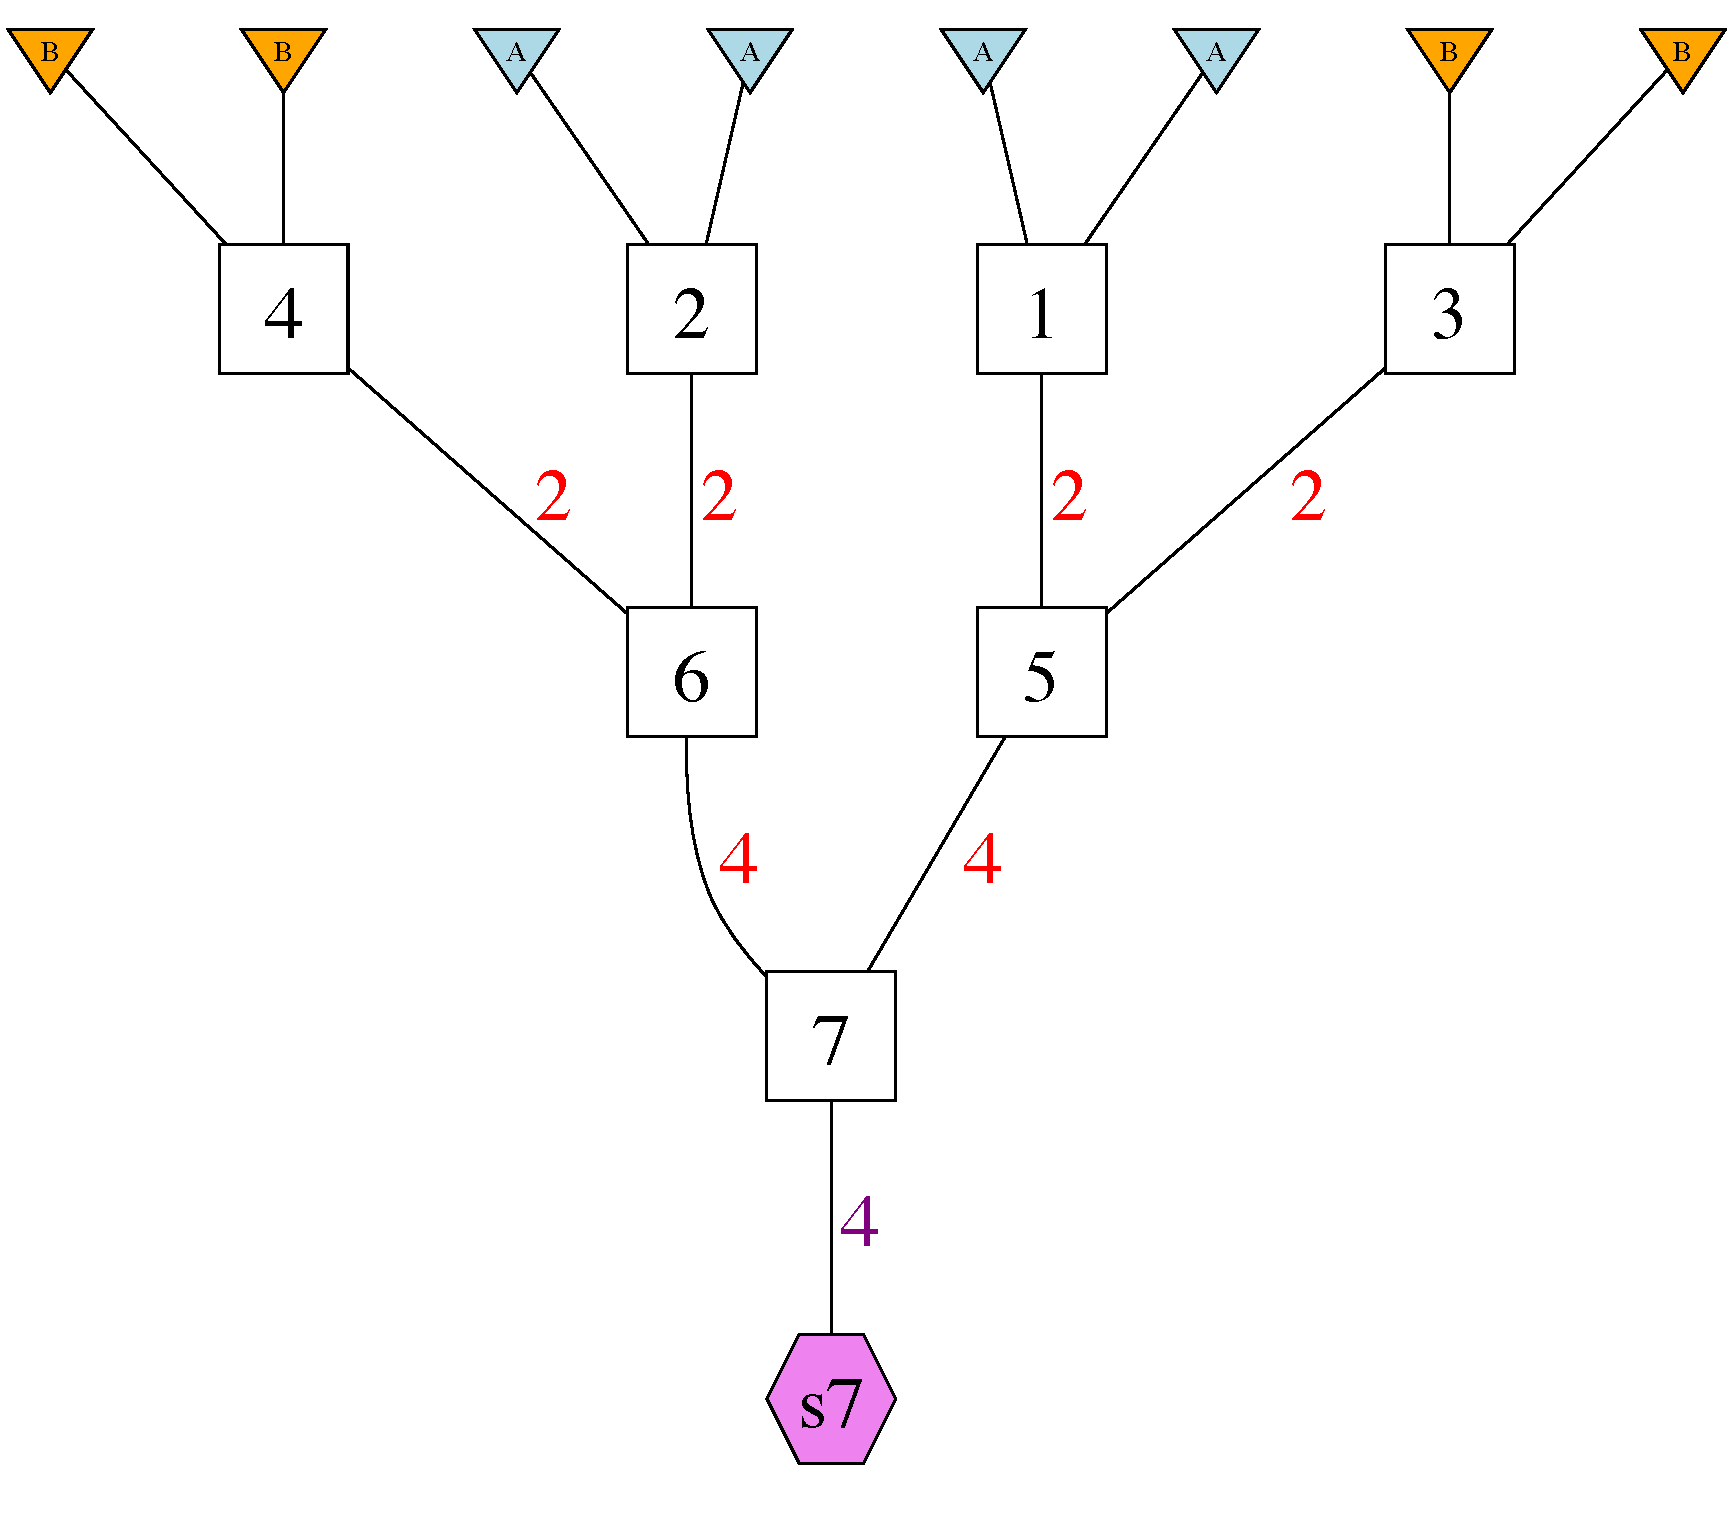
\includegraphics[width=\columnwidth]{figures/F2.pdf}
\end{center}
\caption[\gspcapone]{\gspcapone}
\label{fig:gsp1}
\end{figure}
%%%%%%%%%%%%
It is important to understand that, apart from the founder nodes, the individual
nodes in a GSP do not necessarily represent only a single individual.  Specifically,
since we are preserving all genetic material, multiple gametes may get segregated
through each non-founder node in a GSP\@.

Genetic material is segregated through
a GSP using these steps, done upon each node in an order such that the steps
are run on each node's parents before being run on the node itself:
\begin{enumerate}
\item Each genome in a triangle above a founder node represents a gamete
carrying a single, haploid copy of the genome.
These gametes are united within the founder individual and then
following recombination between each chromosome
with probability $\frac{1}{2}$ and within each chromosome according to
a user-specified recombination map,
 one gamete is assorted down each edge from the founder node to its daughter.
\item Each non-founder node, $x$, will have exactly two edges coming
into it---one from each parent.  Each of the $G^+_{x,1}$ gametes coming in from the
first edge is united with a single one of the $G^+_{x,2}$ gametes coming
in on the second edge (in a random order).
\item If a non-founder node $x$ has an edge to a sample node,
a randomly chosen $S_x$ of the united pairs of gametes are delivered
to the sample node to constitute the $S_x$ samples taken from individual
node $x$. Any remaining united pairs of gametes are treated as in (4) below.
\item United pairs of gametes (including those remaining after delivery
to a sample node) in each non-founder node $x$ are segregated into
gametes with recombination, and each of these gametes is assigned, in
random order, to the gamete edges proceeding downward out of the node,
with the number of gametes assigned to the $i\thh$ downward edge being
$G^-_{x,i}$.
\end{enumerate}
At the end of this process, the samples simulated (as united pairs of gametes)
into the sample nodes will contain all of the genetic material found in the founders (and
no more than that)
but that material will have been segregated and recombined according to the pedigree.  Thus the
samples obtained from a GSP can be simulated with the expected admixture fractions
for any hybrid category that can be specified by a pedigree.  They have also been simulated
in a way that 1) respects physical linkage---each individual inherits segments of the genome
simulated using a recombination map; 2) does not duplicate any genetic material---the sampling of
genetic material is entirely without replacement so it will not induce RIPI; and 3) no genetic material has been lost---all the genetic material of the founders
is represented in the samples, maximizing the number of individuals and markers available to
use in downstream analyses.

In the \gscramble{} package there is a convenience function called {\footnotesize\tt create\_GSP()} that
will create GSPs for samples up to and including second-generation backcrosses (an example appears in Figure~\ref{fig:exampleGSPs}); 
%%%%%
\begin{figure}
\newcommand{\gspcaptwo}{\footnotesize
An example GSP generated by {\footnotesize\tt create\_GSP()} that produces four different
admixture categories: one~$F_1$ in sample node~s7; two~$F_2$'s in sample node~s11; one $BC_1$ in sample node~s9; and two $BC_2$'s in sample node~s10. 
}
\begin{center}
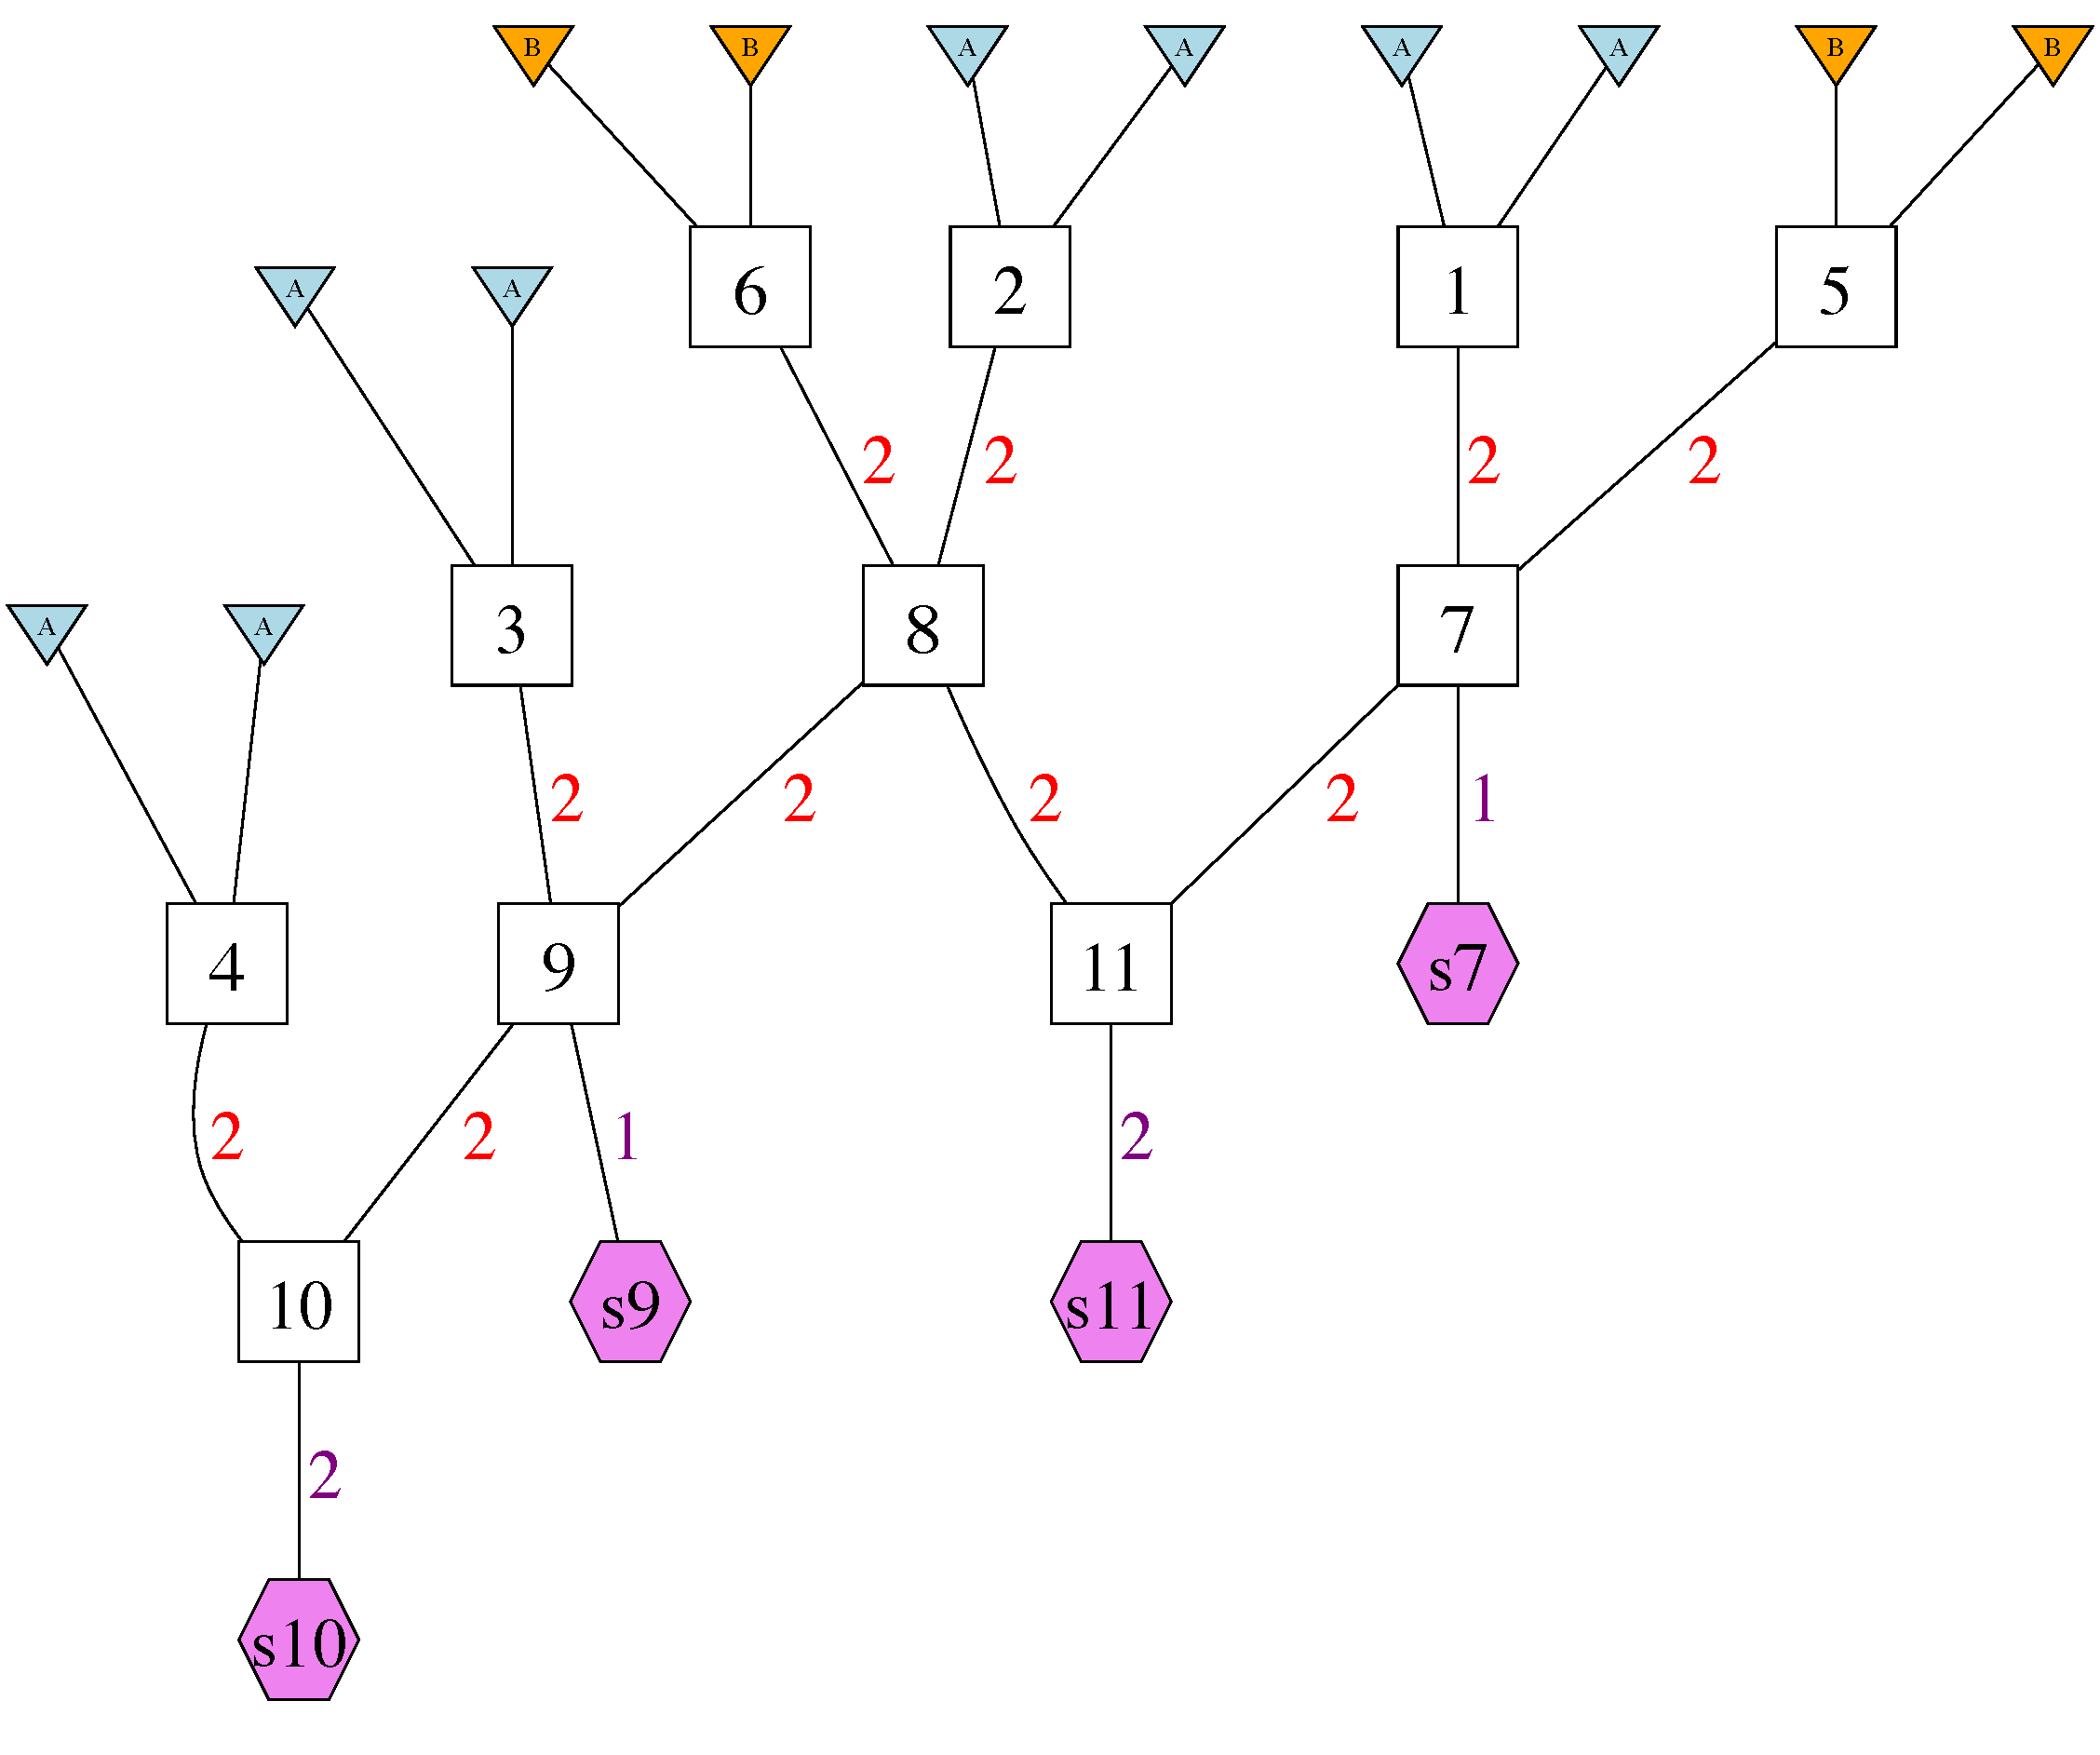
\includegraphics[width=\columnwidth]{figures/AllThem.pdf}
\end{center}
\caption[\gspcaptwo]{\gspcaptwo}
\label{fig:gsp1}
\end{figure}
%%%%
however, \gscramble{} is designed
to handle user-specified GSPs of arbitrary complexity.  When creating one's own GSP, it is useful
to keep in mind a handful of requirements for a GSP to be valid. Writing $\founders$ for the set of all founder nodes, $\nonfound$ for the set of all non-founder nodes, and $\nonfounds$ for all non-founder
nodes that are not parents of other non-founders, but are adjacent to a sample node, $\nonfounde$ for all
non-founder nodes that have non-founder node daughters, but no sample nodes, and $\nonfoundse$ for all
non-founder nodes that are parents of non-founder nodes and also adjacent to sample-nodes, the necessary conditions
for a valid GSP, in addition to having no inbreeding loops, are:
\begin{equation}
\begin{aligned}
\sum_{x \in \nonfounds \cup \nonfoundse} S_x &= |\founders| &  \\
\sum_{i=1}^{e_x} G^-_{x,i} &= 2 & \forall x \in \founders \\
G^+_{x,1} &= G^+_{x,2} & \forall x \in \nonfound \\
\sum_{i=1}^{e_x} G^-_{x,i} &= G^+_{x,1} +  G^+_{x,2} & \forall x \in \nonfounde  \\
 S_x/2 + \sum_{i=1}^{e_x} G^-_{x,i} &= G^+_{x,1} +  G^+_{x,2} & ~~~\forall x \in \nonfoundse.  \\
\end{aligned}
\end{equation}
Before simulating from a GSP, \gscramble{} checks to ensure the GSP
satisfies these validity conditions.  The simulation of genomic segments
from founders to samples in a GSP is performed by the \gscramble{} function
{\footnotesize\tt segregate()}, which requires as input a list of GSPs through which
to segregate genomic segments, and, for each such GSP, a table that maps the
population labels on each GSP (in the inverted triangles atop the founders) to the
different sampled groups of individuals.

\subsection*{Permutation procedures}

\gscramble{} uses a GSP to segregate segments of genetic material from the founders
to the samples.  At the end of segment simulation, the genome of each sample
is recorded as a mosaic of segments that derive from different founders.  In order
to create a data set of markers in each sample, it is necessary only to identify the alleles
that occurred on each segment within the founders and propagate those alleles to the
corresponding segments within the samples.  At the stage of assigning alleles to
founders, \gscramble{} provides a variety of ways to permute alleles amongst
the collection of individuals from which the founders are drawn.  By using permutation,
variability in the data is created, but, since it is done without sampling with replacement, it does
not induce RIPI.

These permutations are executed upon the genotypes provided by the user.
\gscramble{} accepts genetic data as a matrix with $N$ rows (one for each individual) and
$2L$ columns (two for each locus). If the data have been phased, then the phased alleles from the
first haplotype should occupy the
first entry for each locus within an individual, while alleles phased together on the second hapltotype should occupy the
second entry for each locus. 
There can be several populations represented in the data set, but
each individual must belong to exactly one
population.  

Permutation of alleles proceeds within populations, such that
the frequencies of alleles from each population remain the same as those observed
in the samples themselves. Following permutation, there remain individuals
in each population, but the alleles that they carry are different after permutation.  These
individuals are assigned, in order, to be the founders from each population in the GSP. Subsequently,
after genetic material is segregated to the samples, the alleles found on each genomic segment in those permuted
founders are then propagated to the samples.  It is worth noting that this approach allows for simulation
with large genomic data sets, with hundreds of thousands to millions of markers, since segregation
through the pedigree is done by segments, and not on a locus-by-locus basis. The only operations
involving all the alleles in all the individuals are the permutation steps and indexing into the segments,
which may be done efficiently with matrices in R.

Permutation of alleles is handled within the \gscramble{} function {\footnotesize\tt segments2markers()}
which takes as input the segments segregated down a GSP, a matrix of sampled genotypes, and a specification
of the group that each sampled individual belongs to.  The permutation performed when running
{\footnotesize\tt segments2markers()} is controlled by two main options.  The first, {\tt\footnotesize preserve\_individuals},
can take three different values.  If {\tt\footnotesize preserve\_individuals = TRUE}, then entire individuals are permuted,
such that all the alleles within an individual remain together.  If {\tt\footnotesize preserve\_individuals = "BY\_CHROM"}, then
the alleles within an individual found on a homologous pair of chromosomes remain together, but the different
chromosome pairs of an individual are independently permuted into new positions in the data set.  This form of permutation
maintains the LD between markers on the same chromosome, which may be desirable in some contexts.
If {\tt\footnotesize preserve\_individuals = FALSE} then each gene copy within an individual is permuted separately,
providing the maximal scrambling of the data.   The second option, {\tt\footnotesize preserve\_haplotypes}, can take two
different values, {{\tt\footnotesize FALSE} (the default) and {\tt\footnotesize TRUE}.  This option, which keeps alleles together
on the same haplotype, should be set to true only
if the original genotypes are phased into separate haplotypes. 

%%%%%%%
\newcommand{\permcap}{\footnotesize An illustration of how \gscramble{} permutes data under
different options.  {\bf (a)}~A picture
representing an original data set of $N=12$ diploids sampled from three populations and typed at $L=15$ markers. 
Different colors represent different sampled individuals. Individuals 1--5 are shades of blue and green, indicating that they 
are from a single population.  Individuals 6--9 are from another population, (shades of red and orange), while 10--12
are from a third population and are colored shades of violet. Thick vertical black lines separate the different 
populations.  Markers are shown in rows. There are 6 markers on the first chromosome, 5 on the second, and 4 on the 
third.  Each chromosome is delimited by a thick, horizontal black line. The "a" and the "b" in the colored cells denote the first and second gene copies within an individual at each marker.  It is worth noting that this representation shows a $2L \times N$ matrix,
which is the transpose of the $N\times 2L$ matrix used to supply genetic marker data to \gscramble{}. {\bf (b)}~Examples of how the {\tt\footnotesize preserve\_individuals} and {\tt\footnotesize preserve\_haplotypes} options of the {\tt\footnotesize segments2markers()}
function affect the permutation of 
the genetic data of the original data set.  Panel headers show the option values while the colors and "a" and "b" values
in the colored cells show the original position of each gene copy in the original sample.  Note that permutation is always
done within the populations.  When {\tt\footnotesize preserve\_individuals = TRUE},  then just the 
individuals in their entirety are permuted.  When {\tt\footnotesize preserve\_individuals = "BY\_CHROM"}, each pair
of a single chromosome within an individual remains together when permuted. When {\tt\footnotesize preserve\_individuals = FALSE}, gene copies are freely permuted between individuals.  The option {\tt\footnotesize preserve\_haplotypes = TRUE} causes each haplotype on a chromosome to be preserved
while permuting. This option should only be used when the original data set is phased.
}
\begin{figure*}
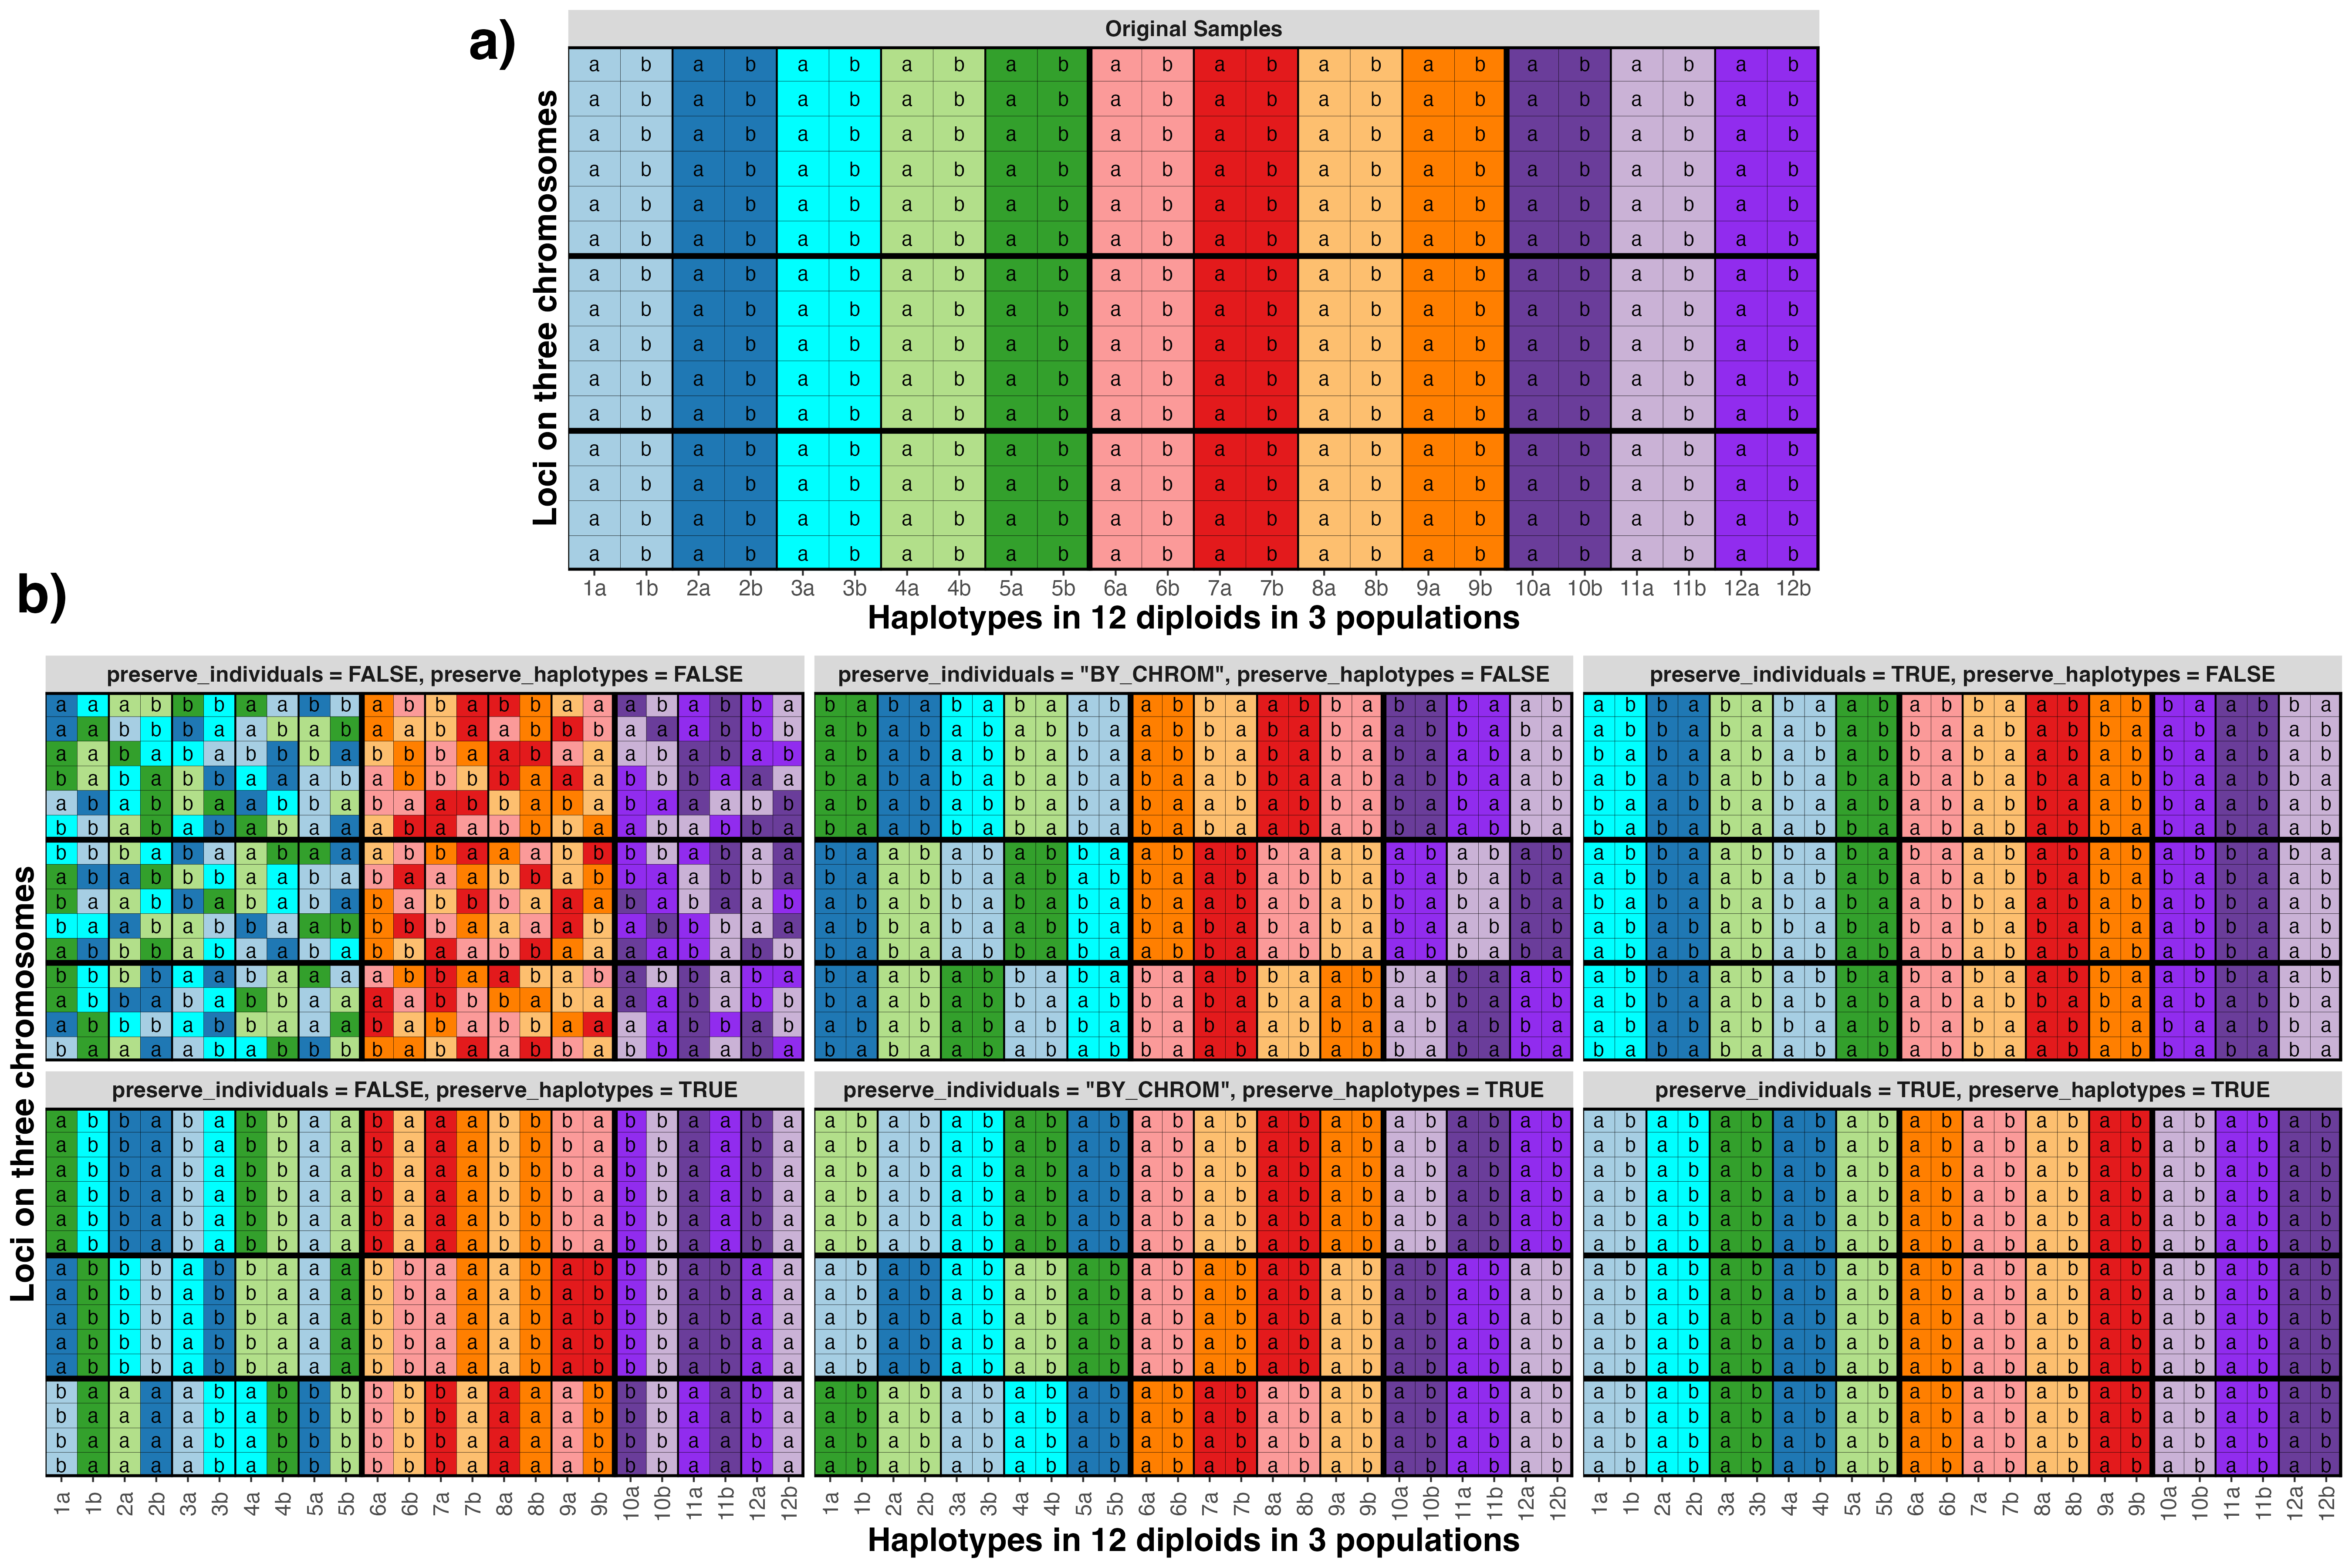
\includegraphics[width=\textwidth]{figures/permutations-plot.png}
\caption[\permcap]{\permcap}
\end{figure*}
%%%%%%%

\subsection*{Empirical Examples}

\subsubsection*{Rainbow/cutthroat trout hybrids in California}

Boing.

\subsubsection*{Feral pigs in Missouri}

Genetic samples were collected from invasive wild pigs across a SPATIAL EXTENT in southeastern Missouri that were lethally removed through population control efforts conducted as a component of the Missouri Feral Hog Elimination Partnership
by US Department of Agriculture – Animal Plant Health Inspection Services – Wildlife Services, Missouri Department of Conservation, and other cooperative state agencies CHECK.
DNA was extracted from hair or tissue (collected from animals at the time of euthanasia) with commercially available magnetic bead recovery kits (MagMax DNA, Thermo Fisher Scientific).
Genotyping was performed with GeneSeek’s Genomic Profiler for Porcine HD which provides 62,128 biallelic SNP loci that are mapped across the 18 autosomal chromosomes.
We implemented standard genotype quality control metrics, specifically, we pruned genotypes with call rates <95\% and minor allele frequencies <5\%.
We implemented linkage disequilibrium (LD) pruning using a window size of 50 loci and step size of 5 loci to remove markers above a linkage threshold of R2 > 0.5.

\gscramble{} REFERENCE GROUPS
\gscramble{} PEDIGREES
ADMIXTURE \gscramble{} VS EMPIRICAL
FST OF EMPIRICAL AND \gscramble{} CORE POPULATIONS






\section*{Results}

\subsection*{An introductory motivating example}

As expected, the perceived ability to estimate $q_A$ with ADMIXTURE was higher
for larger values of $L$ and for smaller values of $N$ (Figure~\ref{fig:bias-sims}).
%%%
\begin{figure*}
\newcommand{\biassimscap}{\footnotesize ADMIXTURE estimates of $q_A$ as described in
{\em An introductory motivating example}. In these results, the apparent ability to estimate $q_A$
is a bias resulting from the use of sampling with replacement to simulate new, admixed genotypes to
test in ADMIXTURE.  In each figure, the different columns represent different numbers of markers
from 10 to 100,000, while different rows represent different original sample sizes, $N$, taken. Colors
of the boxplots indicate how many new individuals, $n$, of each $q_A$ value were simulated during each
replicate.}
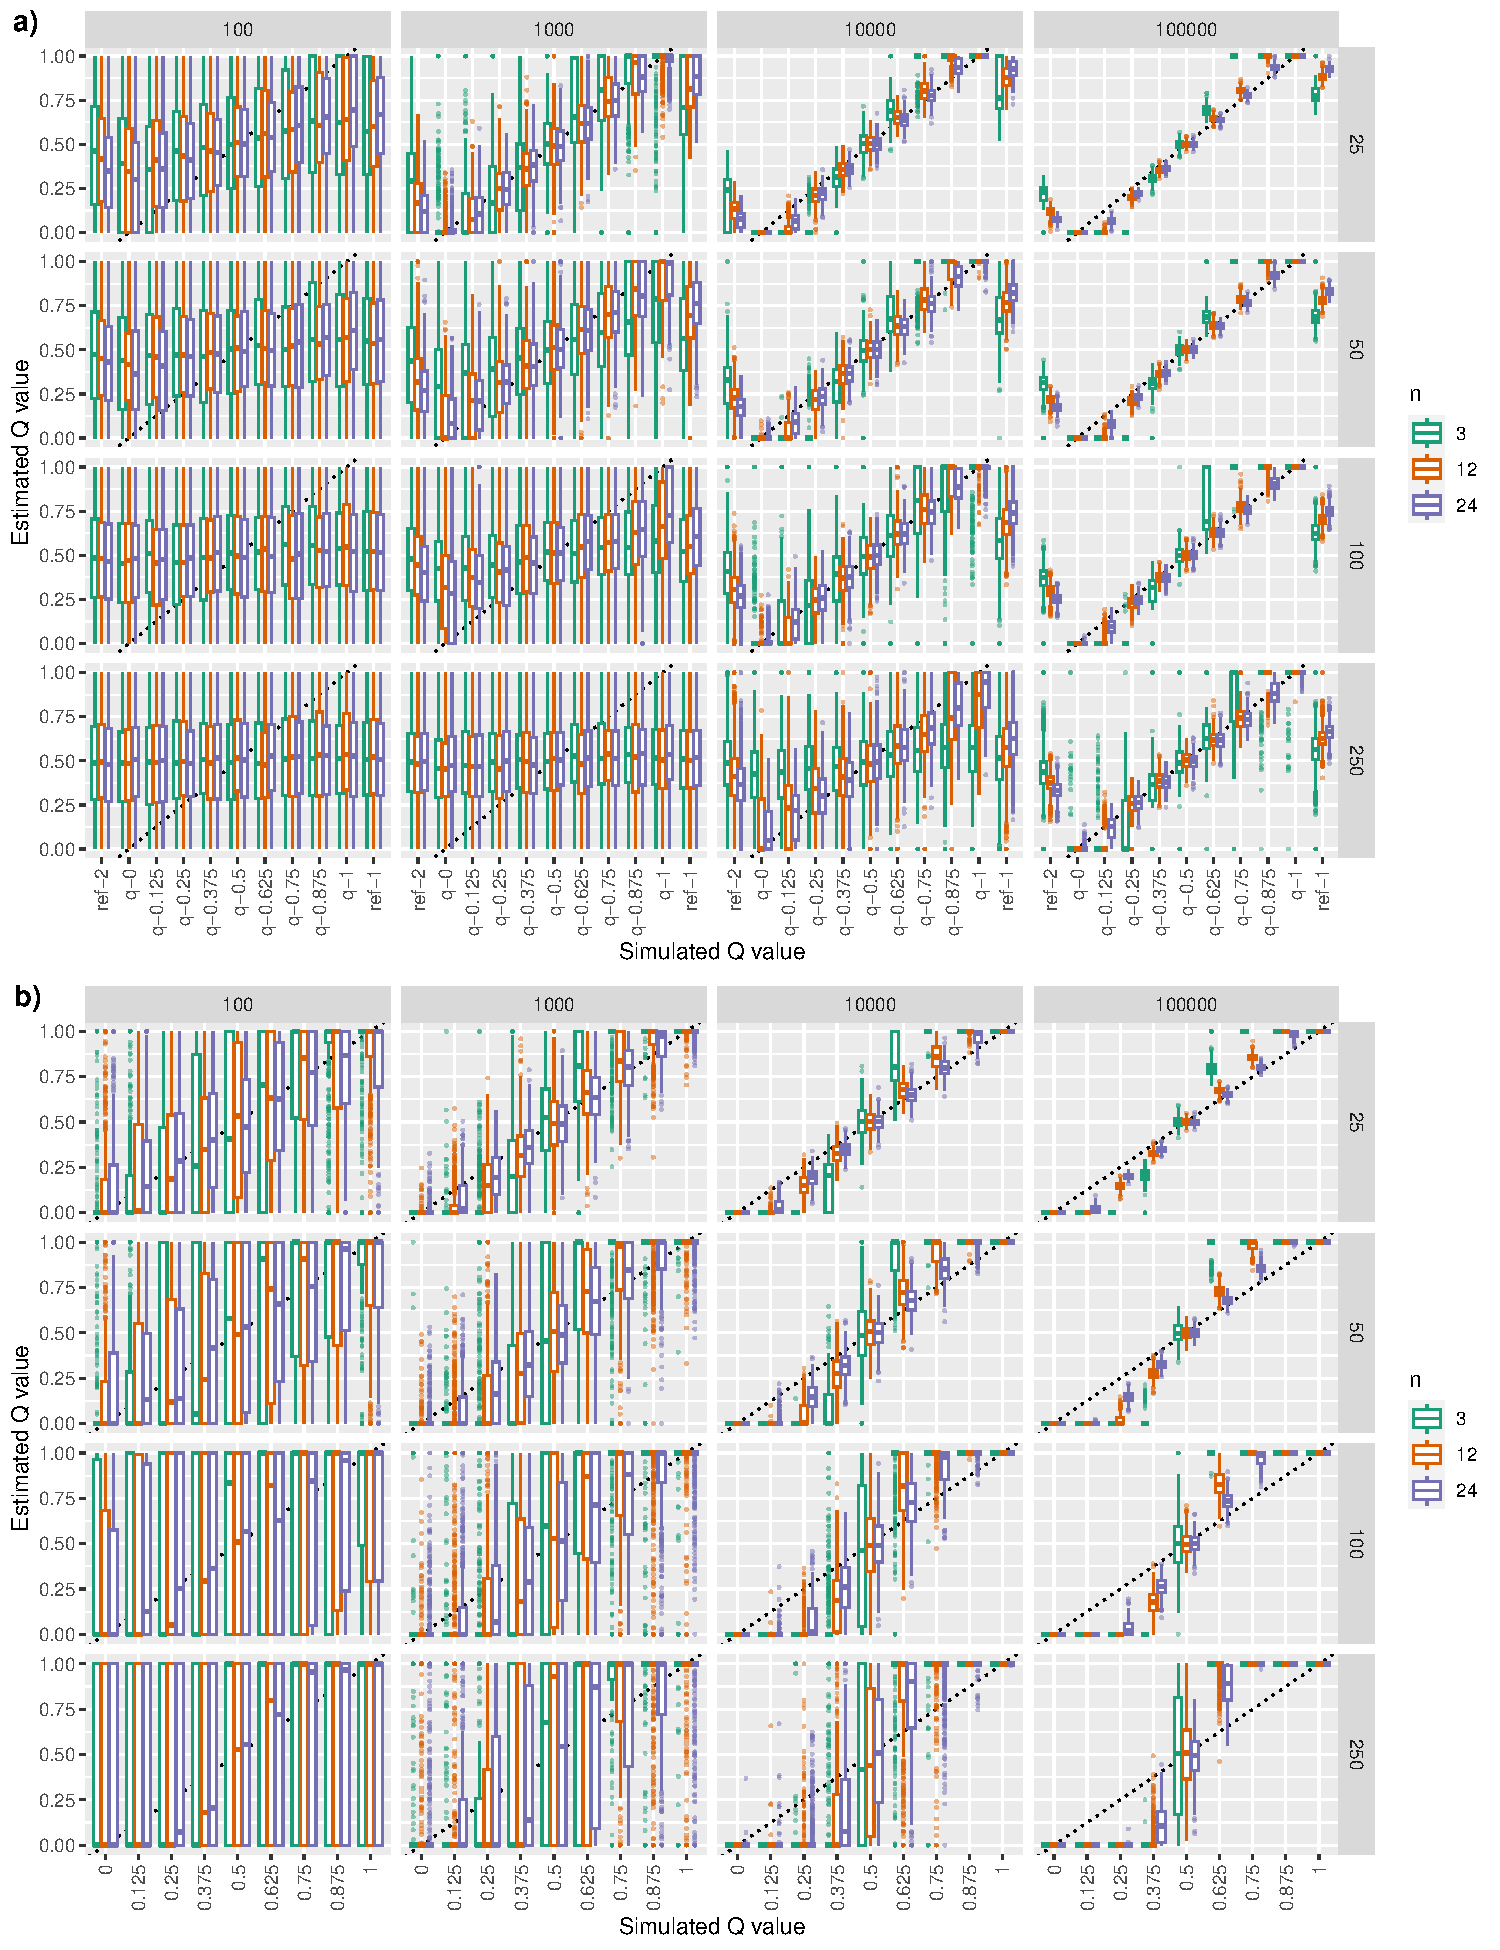
\includegraphics[width=0.96\textwidth]{figures/bias-sims-unsup-and-sup.pdf}
\caption[\biassimscap]{\biassimscap}
\label{fig:bias-sims}
\end{figure*}
%%%
It is interesting to note
that, for numbers of loci,  $L$, that are 100 (or smaller) the effect is observed only when
sample size, $N$, is as small as 25---and even then the effect is slight.  However, when the
number of markers increases to 100,000---values that are becoming commonplace with the availability of chip-
or sequencing-based approaches---it is apparent that the sampling-with-replacement approach
induces an extreme bias.  With 100,000 markers, even if sample sizes ($N$) are as large as 250 individuals,
using na\"{i}ve simulations improperly indicates that admixture fractions of individuals can be
accurately estimated, even when there are no genetic differences, whatsoever between the populations that
samples $A$ and $B$ are drawn.



\section*{Discussion}

Somewhere here I want to mention that the Anderson et al. (2008) approach for simulating
mixtures of genotypes to assess how well one can estimate mixture proportions---the fraction
of individuals from each of a set of baseline or reference populations---allows the user to
simulate, if desired, more genotypes than occur in the reference samples.  This is because
a trick is done in the inference stage to remove the correlation between the simulated individual
and the reference sample, relative to the true population, by removing the simulated individual's
genotypes from its own reference population when calculating the likelihood that its genotype
originated from each of the reference populations.  To do the same when doing simulations for
assessing power using ADMIXTURE or STRUCTURE would require hacking the underlying code
of those programs, which is not desirable.  So, for these cases we have used the sampling
without replacement approach.



\section*{Acknowledgements}
We thank etc. etc.   Contribution number  mHAVEAGAS-003


\section*{Author Contributions}

The gscramble simulation approach grew from discussions between TJS and ECA\@.
ECA, RMG, MGD, and TJS wrote the R package, `gscramble.'   Simulations of bias due to RISPI and
of variance in admixture fractions due to physical linkage were conducted by ECA.
The empirical analyses using `gscramble' were conducted
by MGD and RMG with data from TJS and by ECA with previously published data.  All authors contributed to writing and
editing the manuscript.

\section*{Data Availability Statement}

\begin{itemize}
\item Stable version of \gscramble{} available on CRAN: \url{https://CRAN.R-project.org/package=gscramble}
\item Development version and entire revision history on GitHub: \url{https://github.com/eriqande/gscramble}
\item Online version of all package documentation: \url{https://eriqande.github.io/gscramble}
\item Data and code repository with simulation analyses and steelhead-cutthroat analyses: \url{https://github.com/eriqande/gscramble-paper-sims-and-analyses} (To be transferred to Dryad or Zenodo upon acceptance).
\item Data and code repository for pig analyses: \url{https://github.com/mgdesaix/gscramble-paper-pigs} (To be transferred to Dryad or Zenodo upon acceptance)
\end{itemize}
\mbox{}



\renewcommand{\baselinestretch}{1.0}\normalsize
\bibliography{citation}
\bibliographystyle{men}

\renewcommand{\baselinestretch}{1.66}\normalsize
\section*{Author Contributions}

The gscramble simulation approach grew from discussions between TJS and ECA\@.
ECA, RMG, MGD, and TJS wrote the R package, `gscramble.'   Simulations of bias due to RISPI and
of variance in admixture fractions due to physical linkage were conducted by ECA.
The empirical analyses using `gscramble' were conducted
by MGD and RMG with data from TJS and by ECA with previously published data.  All authors contributed to writing and
editing the manuscript.

\section*{Data Availability Statement}

\begin{itemize}
\item Stable version of \gscramble{} available on CRAN: \url{https://CRAN.R-project.org/package=gscramble}
\item Development version and entire revision history on GitHub: \url{https://github.com/eriqande/gscramble}
\item Online version of all package documentation: \url{https://eriqande.github.io/gscramble}
\item Data and code repository with simulation analyses and steelhead-cutthroat analyses: \url{https://github.com/eriqande/gscramble-paper-sims-and-analyses} (To be transferred to Dryad or Zenodo upon acceptance).
\item Data and code repository for pig analyses: \url{https://github.com/mgdesaix/gscramble-paper-pigs} (To be transferred to Dryad or Zenodo upon acceptance)
\end{itemize}
\mbox{}




\newpage
\renewcommand{\baselinestretch}{1.0}\normalsize
\listoffigures
\newpage

\end{document}
